\let\lesson\undefined
\newcommand{\lesson}{\phantomlesson{Bài 9.}}
\setcounter{section}{2}
\section{Bài tập trắc nghiệm}
\begin{enumerate}[label=\bfseries Câu \arabic*:,leftmargin=1.5cm]
	\item \mkstar{1}
	
	
	{Một vật được ném ngang từ độ cao $h$ so với mặt đất với vận tốc ném là $v_0$. Kết luận nào sau đây đúng?
		\begin{mcq}(2)
			\item Vận tốc khi tiếp đất hướng thẳng đứng xuống dưới.
			\item Thời gian bay phụ thuộc vào $h$.
			\item Tầm bay xa không phụ thuộc vào $h$.
			\item Thời gian bay phụ thuộc vào $v_0$
		\end{mcq}
	}
	
	\hideall
	{	\textbf{Đáp án: B.}
	}
	
	\item \mkstar{1}
	
	
	{Ở nơi có gia tốc rơi tự do là $g$, từ độ cao $h$ so với mặt đất, một vật được ném ngang với tốc độ ban đầu $v$. Tầm bay xa của vật là
		\begin{mcq}(4)
			\item $L=v\sqrt{\dfrac{h}{2g}}$.
			\item $L=v\dfrac{2h}{g}$.
			\item $L=v\dfrac{h}{2g}$.
			\item $L=v\sqrt{\dfrac{2h}{g}}$.
		\end{mcq}
	}
	
	\hideall
	{	\textbf{Đáp án: D.}
		
		Tầm bay xa của vật ném ngang tính theo công thức $L=v\sqrt{\dfrac{2h}{g}}$.
	}
	\item \mkstar{2}
	
	
	{Hai vật ở cùng một độ cao, vật I được ném ngang với vận tốc đầu $v_0$, cùng lúc đó vật II được thả rơi không vận tốc đầu. Bỏ qua sức cản của không khí. Kết luận nào sau đây là đúng?
		\begin{mcq}(2)
			\item Vật I chạm đất trước vật II.
			\item Thời gian rơi phụ thuộc vào khối lượng mỗi vật.
			\item Vật I chạm đất sau vật II.
			\item Vật I chạm đất cùng lúc với vật II.
		\end{mcq}
	}
	
	\hideall
	{	\textbf{Đáp án: D.}	
		
		Theo công thức tính thời gian chuyển động của vật ném ngang, ta thấy đó cũng là công thức tính thời gian vật rơi tự do nếu được thả từ cùng độ cao. Vậy hai vật chạm đất cùng lúc.
	}
	
	\item \mkstar{2}\\
	{Quỹ đạo chuyển động của vật ném ngang là một
		\begin{mcq}(4)
			\item đường thẳng.
			\item đường tròn.
			\item đường xoáy ốc.
			\item nhánh parabol.
		\end{mcq}
	
}
\hideall{
\textbf{Đáp án: D.}
}

\item \mkstar{2}\\
{Từ trên một máy bay đang chuyển động đều theo phương nằm ngang người ta thả một vật rơi xuống đất. Bỏ qua sức cản không khí. Nhận xét nào sau đây là sai?
	\begin{mcq}
		\item Người quan sát đứng trên mặt đất nhìn thấy quỹ đạo của vật là một phần của parabol.
		\item Người quan sát đứng trên máy bay nhìn thấy quỹ đạo của vật là một phần của parabol.
		\item Người quan sát đứng trên máy bay nhìn thấy quỹ đạo của vật là một đường thẳng đứng.
		\item Vị trí chạm đất ở ngay dưới máy bay theo phương thẳng đứng.
	\end{mcq}

}
\hideall{
\textbf{Đáp án: B.}\\
Máy báy và vật có cùng vận tốc trên phương ngang, do đó người trên máy bay thấy quỹ đạo của vật là một đường thẳng đứng.
}
	
	
	\item	\mkstar{2}\\
	{Trong chuyển động ném ngang, gia tốc của vật tại một vị trí bất kì luôn có đặc điểm là hướng theo
	\begin{mcq}(2)
		\item phương ngang, cùng chiều chuyển động.
		\item phương ngang, ngược chiều chuyển động.
		\item phương thẳng đứng, chiều từ dưới lên trên.
		\item phương thẳng đứng, chiều từ trên xuống dưới.
	\end{mcq}
}
\hideall{
\textbf{Đáp án: D.}
}

\item \mkstar{3}\\
{Một vật ở độ cao $h$ được ném theo phương ngang với tốc độ $v_0$ và rơi chạm đất sau $\SI{5}{\second}$. Lấy $g=\SI{10}{\meter/\second^2}$. Vật được ném từ độ cao
	\begin{mcq}(4)
		\item $\SI{100}{\meter}$.
		\item $\SI{125}{\meter}$.
		\item $\SI{200}{\meter}$.
		\item $\SI{30}{\meter}$.
	\end{mcq}

}
\hideall{
\textbf{Đáp án: B.}\\
$$H=\dfrac{1}{2}gt^2=\SI{125}{\meter}.$$
}

\item \mkstar{3}\\
{Một vật ở độ cao h được ném theo phương ngang với tốc độ $v_0 = \SI{50}{\meter/\second}$ và rơi chạm đất sau $\SI{10}{\second}$. Lấy $g = \SI{10}{\meter/\second^2}$. Tầm xa của vật là
\begin{mcq}(4)
	\item $\SI{400}{\meter}$.
	\item $\SI{500}{\meter}$.
	\item $\SI{300}{\meter}$.
	\item $\SI{200}{\meter}$.
\end{mcq}
}
\hideall{
\textbf{Đáp án: B.}\\
Tầm xa của vật ném ngang:
$$L=v_0\cdot t=\SI{500}{\meter}.$$
}

\item \mkstar{3}\\
{Một quả bóng được ném theo phương ngang với vận tốc ban đầu $v_0 = \SI{20}{\meter/\second}$ từ độ cao $\SI{45}{\meter}$. Lấy $g = \SI{10}{\meter/\second^2}$. Bỏ qua sức cản không khí. Tầm bay xa của quả bóng là
\begin{mcq}(4)
	\item $\SI{30}{\meter}$.
	\item $\SI{45}{\meter}$.
	\item $\SI{60}{\meter}$.
	\item $\SI{90}{\meter}$.
\end{mcq}
}
\hideall{
\textbf{Đáp án: C.}\\
Tầm bay xa của quả bóng:
$$L=v_0\cdot\sqrt{\dfrac{2H}{g}}=\SI{60}{\meter}.$$
}

	\item \mkstar{3}
	
	
	{Một máy bay trực thăng cứu trợ với vận tốc không đổi $v_0$ theo phương ngang ở độ cao $1500\ \text m$ so với mặt đất. Máy bay chỉ có thể tiếp cận được khu vực cách điểm cứu trợ $2\ \text{km}$ theo phương ngang. Lấy $g=9,8\ \text {m/s}^2$. Để hàng cứu trợ được thả đúng nơi cần máy bay phải bay với vận tốc bằng
		\begin{mcq}(4)
			\item $114,31\ \text{m/s}$.
			\item $11,431\ \text{m/s}$.
			\item $228,62\ \text{m/s}$.
			\item $22,86\ \text{m/s}$.
		\end{mcq}
	}
	
	\hideall
	{	\textbf{Đáp án: A.}
		
		Hàng cứu trợ được thả từ máy bay chuyển động ném ngang.
		
		Áp dụng công thức tính tầm bay xa:
		\[L=v_0\sqrt{\dfrac{2h}{g}}\]
		
		Suy ra $v_0 = \dfrac{L}{\sqrt{\dfrac{2h}{g}}}=114,31\ \text{m/s}$.
	}

\item \mkstar{3}\\
{Một vật được ném ngang với vận tốc $v_0 = \SI{30}{\meter/\second}$, ở độ cao $h = \SI{80}{\meter}$. Lấy $g=\SI{10}{\meter/\second^2}$. Tầm bay xa và tốc độ của vật khi chạm đất là
\begin{mcq}(2)
	\item $\SI{120}{\meter}$; $\SI{50}{\meter/\second}$.
	\item $\SI{50}{\meter}$; $\SI{120}{\meter/\second}$.
	\item $\SI{120}{\meter}$; $\SI{70}{\meter/\second}$.
	\item $\SI{70}{\meter}$; $\SI{120}{\meter/\second}$.
\end{mcq}
}
\hideall{
\textbf{Đáp án: A.}\\
Tầm bay xa của vật:
$$L=v_0\cdot\sqrt{\dfrac{2h}{g}}=\SI{120}{\meter}$$
Tốc độ của vật khi chạm đất:
$$v=\sqrt{v^2_0+2gh}=\SI{50}{\meter/\second}.$$
}
	
	\item \mkstar{4}
	
	
	{Ném vật theo phương ngang với vận tốc $10\ \text{m/s}$ từ độ cao $40\ \text m$ xuống đất. Lấy $g=10\ \text{m/s}^2$. Phương trình quỹ đạo và tọa độ của vật sau $2\ \text s$ là
		\begin{mcq}(2)
			\item $y=\dfrac{x^2}{50}\ \text m$ và $x=50\ \text m$; $y=20\ \text m$.
			\item $y=\dfrac{x^2}{20}\ \text m$ và $x=50\ \text m$; $y=20\ \text m$.
			\item $y=\dfrac{x^2}{20}\ \text m$ và $x=20\ \text m$; $y=20\ \text m$.
			\item $y=\dfrac{x^2}{50}\ \text m$ và $x=20\ \text m$; $y=20\ \text m$.
		\end{mcq}
	}
	
	\hideall
	{	\textbf{Đáp án: C.}
		
		Phương trình quỹ đạo:
		\[y=\dfrac{g}{2v_0^2}x^2 = \dfrac{10}{\cdot 10^2}x^2 = \dfrac{x^2}{20}\]
		
		Tọa độ vật sau $2\ \text s$:
		\[x=v_0 t = 20\ \text m\]
		\[y=\dfrac{1}{2}gt^2 = 20\ \text m\]
	}
\end{enumerate}
\section{Bài tập tự luận}
\begin{enumerate}[label=\bfseries Bài \arabic*:,leftmargin=1.5cm]
	\item \mkstar{2}
	
	
	{Ném vật theo phương ngang ở độ cao $50\ \text m$ so với mặt đất, lấy $g=9,8\ \text{m/s}^2$. Vận tốc lúc ném là $18\ \text{m/s}$. Tính thời gian từ lúc ném cho đến khi vật chạm đất và tầm xa của vật.
	}
	
	\hideall
	{
		Thời gian vật rơi:
		$$t=\sqrt{\dfrac{2h}{g}}=\SI{3.2}{\second}.$$
		Tầm xa của vật:
		$$L=v_0t=\SI{57.6}{\meter}.$$
		
		Vậy thời gian rơi là $t=3,2\ \text s$, tầm xa là $\SI{57.6}{\meter}$.
	}

\item \mkstar{2}\\
Một hòn đá được ném từ đỉnh của một vách đá thẳng đứng, cao $\SI{45}{\meter}$ so với mặt đất, với vận tốc ban đầu có độ lớn $\SI{15}{\meter/\second}$ theo phương ngang. Mất bao lâu để hòn đá đến mặt đất? Nó cách chân vách đá bao xa khi chạm đất?
\begin{center}
	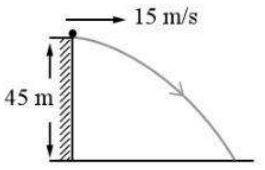
\includegraphics[width=0.2\linewidth]{../figs/VN10-2022-PH-TP012-P-1}
\end{center}
\hideall{
Thời gian hòn đá chạm đất:
$$t=\sqrt{\dfrac{2h}{g}}=\SI{3}{\second}.$$
Tầm xa của hòn đá:
$$L=v_0t=\SI{30}{\meter}.$$
}

	\item \mkstar{3}
	
	
	{Một hòn bi lăn dọc theo một cạnh của một mặt bàn hình chữ nhật nằm ngang cao $h=1,25\ \text m$. Khi ra khỏi mép bàn, nó rơi xuống nền nhà tại điểm cách mép bàn $L=1,5\ \text m$ (theo phương ngang). Lấy $g=10\ \text{m/s}^2$. Tính thời gian hòn bi rơi và tốc độ của hòn bi khi rời khỏi mép bàn.
	}
	
	\hideall
	{	Hòn bi ra khỏi mép bàn thì chuyển động ném ngang.
		
		Thời gian hòn bi rơi:
		$$t=\sqrt{\dfrac{2h}{g}}=\SI{0.5}{\second}.$$
		Tốc độ của hòn bi khi rời khỏi mép bàn:
		$$v_0=\dfrac{L}{t}=\SI{3}{\meter/\second}.$$
		Vậy thời gian hòn bi rơi là $\SI{0.5}{\second}$ và tốc độ của hòn bi khi rời khỏi mép bàn là $\SI{3}{\meter/\second}$.
	}
	\item \mkstar{3}
	
	
	{Một vật được ném theo phương ngang với tốc độ $v_0 = 10\ \text{m/s}$ từ độ cao $h$ so với mặt đất. Chọn hệ trục tọa độ $\text Oxy$ sao cho gốc O trùng với vị trí ném, $\text O x$ theo chiều vận tốc đầu, $\text Oy$ hướng thẳng đứng xuống dưới, gốc thời gian là lúc ném. Lấy $g=10\ \text{m/s}^2$. Tìm phương trình quỹ đạo của vật.
	}
	
	\hideall
	{	Phương trình quỹ đạo $y=\dfrac{g}{2v_0^2}x^2 = 0,05x^2$
		
		(Chú ý phân biệt giữa phương trình quỹ đạo $y(x)$ và phương trình chuyển động $y(t); x(t)$)
	}
	
	\item \mkstar{3}\\
	{Một vận động viên ném một quả bóng chày với tốc độ $\SI{90}{\kilo\meter/\hour}$ từ độ cao $\SI{1.75}{\meter}$. Giả sử quả bóng chày được ném ngang, lực cản không khí là không đáng kể và lấy $g=\SI{9.8}{\meter/\second^2}$.
		\begin{enumerate}[label=\alph*)]
			\item Viết phương trình chuyển động của quả bóng chày theo hai 	trục $Ox$ và $Oy$.
			\item Quả bóng chày đạt tầm xa bao nhiêu? Tính tốc độ của quả bóng ngay trước khi chạm đất.
		\end{enumerate}
	
}
\hideall{
\begin{enumerate}[label=\alph*)]
	\item \begin{align*}
		\begin{cases}
			x=25t \left(\si{\meter}\right)\\
			y=4,9t^2 \left(\si{\meter}\right)
		\end{cases}
	\end{align*}
\item $L\approx\SI{14.94}{\meter}$.\\
Tốc độ của quả bóng trước khi chạm đất $v\approx\SI{25.68}{\meter/\second}$.
\end{enumerate}
}
	
	
\item \mkstar{3}\\
Một chiếc máy bay muốn thả hàng tiếp tế cho những người leo núi đang bị cô lập. Máy bay đang bay ở độ cao $\SI{235}{\meter}$ so với vị trí đứng của những người leo núi với tốc độ $\SI{250}{\kilo\meter/\hour}$ theo phương ngang. Máy bay phải thả hàng tiếp tế ở vị trí cách những người leo núi bao xa để họ có thể nhận được hàng? Lấy $g=\SI{9.8}{\meter/\second^2}$ và bỏ qua lực cản của không khí.
\begin{center}
	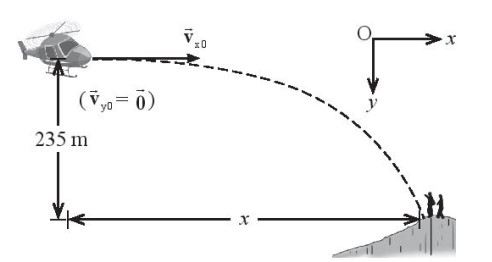
\includegraphics[width=0.5\linewidth]{../figs/VN10-2022-PH-TP012-P-2}
\end{center}
\hideall{
Tầm xa để thả hàng:
$$L=v_0\sqrt{\dfrac{2h}{g}}\approx\SI{481}{\meter}.$$
}
\end{enumerate}